\documentclass[11pt]{article}

% Change "review" to "final" to generate the final (sometimes called camera-ready) version.
% Change to "preprint" to generate a non-anonymous version with page numbers.
\usepackage[final]{acl}

% Standard package includes
\usepackage{times}
\usepackage{latexsym}
\usepackage{amsmath}

% For proper rendering and hyphenation of words containing Latin characters (including in bib files)
\usepackage[T1]{fontenc}
% For Vietnamese characters
% \usepackage[T5]{fontenc}
% See https://www.latex-project.org/help/documentation/encguide.pdf for other character sets

% This assumes your files are encoded as UTF8
\usepackage[utf8]{inputenc}

% This is not strictly necessary, and may be commented out,
% but it will improve the layout of the manuscript,
% and will typically save some space.
\usepackage{microtype}

% This is also not strictly necessary, and may be commented out.
% However, it will improve the aesthetics of text in
% the typewriter font.
\usepackage{inconsolata}

%Including images in your LaTeX document requires adding
%additional package(s)
\usepackage{graphicx}

% If the title and author information does not fit in the area allocated, uncomment the following
%
%\setlength\titlebox{<dim>}
%
% and set <dim> to something 5cm or larger.

\title{Consensus without Accuracy: Investigating LLMs Ability to Recover Item Difficulty Using Paired Comparisons}

\author{Michael L. Chrzan \\
  Center for Educational Data Science \\
  and Innovation, \\
  University of Maryland \\\And
  Benjamin W. Domingue \\
  Stanford University
  \thanks{\textbf{Correspondence:} \href{mailto:mlchrzan@umd.edu}{\texttt{mlchrzan@umd.edu}}}
}

\begin{document}
\maketitle

\begin{abstract}
Large language models (LLMs) offer a scalable way to estimate item difficulty before respondent data are available, but it is unclear whether they can provide reliable estimates, either alone or in aggregate. We evaluate seven frontier LLMs on pairwise comparisons of items from seven datasets with respondent-calibrated one-parameter item response theory (1PL IRT) difficulty estimates. We aggregate their judgments using a hierarchical Bayesian Bradley--Terry model that estimates shared item strengths while accounting for model-specific discrimination and presentation-order bias. The pooled rankings recover a meaningful but incomplete difficulty signal: standardized hierarchical Bradley--Terry strengths correlate moderately with IRT difficulty overall (Spearman's $\rho=0.400$, $p<.001$), with dataset-level correlations ranging from $0.250$ to $0.591$. This heterogeneity persists despite high inter-model agreement (Krippendorff's $\alpha=0.834$--$0.917$) and generally high within-model triplet transitivity, demonstrating that consensus and internal consistency do not guarantee external psychometric validity. The hierarchical model also reveals substantial variation in rater discrimination and position bias, while in-sample predictive accuracy ranges from $0.732$ to $0.874$ across datasets. These findings support LLM pairwise comparisons as a scalable source of provisional item ordering, but not as a replacement for respondent-based calibration.
\end{abstract}

\section{Introduction}
\label{sec:intro}

Item calibration - the process of estimating psychometric properties such as item difficulty - is central to educational assessment but resource-intensive, typically requiring large samples of student response data and extended field-testing periods creating barriers for low-resource testing programs, early-stage item development, and rapid test assembly contexts \citep{jiangSampleSizeRequirements2016}. Recent advances in large language model (LLM) capabilities raise an intriguing question: can item difficulty be meaningfully estimated directly from item text, without recourse to any response data? Such an approach would offer immediate practical utility for item writers and test developers seeking a scalable first-pass difficulty signal for item screening, ordering, or rough-cut form assembly before formal calibration. Prior work has explored LLMs for automated item generation and scoring \citep{vondavierComputationalPsychometricsNew2022}, but their deployment as a calibration proxy for estimating the psychometric difficulty of items never yet administered remains less examined as does the extent to which paired comparisons aid in that effort.
 
Recent work by \citet{wuConceptGuidedChainofThoughtPrompting2024} introduced concept-guided chain-of-thought (CGCoT) prompting as a generalizable framework for scoring texts on latent constructs. CGCoT pairs a sequence of researcher-crafted prompts, each probing a different facet of the latent construct of interest, with LLM-based pairwise comparisons aggregated into a continuous score via the Bradley-Terry (BT) model \citep{bradleyRankAnalysisIncomplete1952}. Originally validated for scaling political affect in social media, CGCoT's structure maps naturally onto item difficulty estimation: an item's text can be characterized through prompts targeting cognitive demand and required ability level, with pairs of items compared by an LLM to establish an ordinal difficulty ranking without any examinee data.

Further, pairwise comparison methods offer a natural interface for eliciting difficulty judgments from LLMs. Rather than requiring absolute estimates - which are psychometrically undefined without a response scale and shown to be unreliable for LLMs \citep{lichtMeasuringScalarConstructs2025} - pairwise comparisons ask a model to make relative judgments, which can then be aggregated into difficulty rankings using models such as the Bradley-Terry model. This approach also allows reliability to be assessed via extensions of Bradley-Terry methods, such as a Hierarchical Bradley-Terry Model \citep{bockenholtHierarchicalModelingPaired2001}, and internal consistency metrics such as triplet transitivity. However, whether LLM-derived BT scores actually align with psychometrically validated difficulty estimates from Item Response Theory (IRT) remains an open empirical question.

\subsection{Contributions}
\label{subsec:contributions}

This study makes three contributions. First, we provide a multi-model, multi-dataset evaluation of whether LLM pairwise judgments recover respondent-calibrated item difficulty. Across seven LLMs and seven educational item sets, the pooled ranking captures a meaningful but incomplete difficulty signal (overall Spearman's $\rho=0.400$), with substantial variation across datasets ($\rho=0.250$--$0.591$).

Next, we aggregate judgments with a hierarchical Bayesian Bradley--Terry model that estimates a shared item-difficulty ranking while separating model-specific discrimination from presentation-order bias. This formulation quantifies uncertainty in the pooled ranking and reveals consequential differences among LLM raters that a simple consensus score would obscure.

Lastly, we distinguish three often-conflated properties of LLM judgments: within-model transitivity, inter-model agreement, and external psychometric validity. Despite generally high transitivity and uniformly high inter-model agreement, alignment with 1PL difficulty remains moderate and heterogeneous, showing that consistent LLM consensus is useful for provisional item ordering but cannot substitute for respondent-based calibration.

\section{Related Work}
\label{sec:related}

The foundational IRT model utilized in large-scale calibration is the 1-Parameter Logistic (1PL) model, commonly known as the Rasch model, introduced by Georg Rasch in 1960 \citep{zotero-item-1169, kolesnikovaEstimatingItemDifficulty2026}. The Rasch model conceptualizes the probability that a specific student correctly answers a specific item as a logistic function of the difference between the student's latent ability and the item's latent difficulty. In generalized terms, if a student's ability exactly matches the item's difficulty, the theoretical probability of a correct response is precisely fifty percent. In traditional workflows, estimating this difficulty parameter requires administering the item to highly calibrated populations whose abilities form a known distribution \citep{feliceBritishCouncilSubmission}. However, when new assessment items are generated, their parameters are entirely unknown, creating what is known as the cold-start problem \citep{wainerComputerizedAdaptiveTesting2000}. If LLMs or machine learning ensembles can accurately predict the difficulty parameter based solely on item content, these synthetic estimates can be used to jump-start the IRT calibration process. This permits the immediate deployment of new items in live environments and vastly reduces the volume of human response data required to achieve statistical stability.

An intuitive methodology for applying LLMs to predict item difficulty is direct absolute estimation. In this paradigm, a language model is provided with the text of an item—including the question stem, correct answer, and distractors—and is instructed via a zero-shot prompt to output a numeric difficulty score or a categorical difficulty level \citep{kolesnikovaEstimatingItemDifficulty2026}. This approach relies on the implicit assumption that the LLM contains a holistic, internally calibrated representation of cognitive complexity that perfectly mirrors human populations. Recent literature indicates that this assumption is fundamentally flawed and suggests that direct absolute judgment by LLMs is fraught with inconsistencies and severe predictive limitations \citep{lichtMeasuringScalarConstructs2025, wangCanLLMsReally2026}. 

To overcome the inherent limitations of direct absolute prediction, researchers have achieved state-of-the-art results by fundamentally altering the LLM's role within the predictive architecture. Rather than acting as a final psychometric judge, the LLM is repositioned as a highly advanced feature extractor \citep{kolesnikovaEstimatingItemDifficulty2026}. In this paradigm, the model is prompted to evaluate specific linguistic, structural, and pedagogical characteristics of the item text. These extracted qualitative features are then fed into traditional supervised machine learning algorithms to predict the final difficulty parameter. By decoupling the semantic extraction (handled by the LLM) from the regression task (handled by ensemble trees like Random Forests and Gradient Boosting algorithms), the predictive system successfully sidesteps the LLM's inability to globally scale difficulty \citep{feliceBritishCouncilSubmission}.

While feature-based ensembles and synthetic simulations provide robust solutions, extracting dozens of qualitative features per item can be computationally expensive, highly prompt-intensive, and strictly domain-dependent. An alternative, highly effective psychometric strategy leverages the language model's fundamental capacity for relative reasoning: pairwise (paired) comparisons. While assigning an isolated assessment item a difficulty score of 7.8 out of 10 requires a stable internal standard, precise calibration against prior examples, and a consistent, unshifting interpretation of what the numerical scale is meant to represent \citep{digiuseppeScalingOpenEndedSurvey2026}, pairwise comparisons ask a significantly simpler question: Which of these two items is more difficult? \citep{kolesnikovaEstimatingItemDifficulty2026}. This localized, relative judgment completely removes the need for a global numerical frame. It severely mitigates anchoring bias, allows for high-resolution discrimination between items of similar complexity, and demonstrates remarkable stability across various LLM architectures and model sizes \citep{digiuseppeScalingOpenEndedSurvey2026}. By transforming the task from an absolute regression to a binary relative choice, the system extracts the model's highest-confidence judgments and has been shown to be highly effective in recent work examining mathematics tasks \citep{kolesnikovaEstimatingItemDifficulty2026}.

However, when utilizing multiple different LLMs or deploying varying prompt architectures to generate large-scale pairwise comparisons the reliability of the artificial "judges" inherently fluctuates. Inspired by the established Crowd-BT algorithm \citep{chenPairwiseRankingAggregation2013}—which automatically estimates the underlying reliability of human crowdsource workers and flags annotators with low quality for removal—researchers have introduced the BT-$\sigma$ model, which extends the traditional Bradley-Terry framework specifically for the "LLM-as-a-jury" setting \citep{qianWhoCanWe2026}. The BT-$\sigma$ Bayesian model introduces a specific discrimination parameter ($\sigma_k$) for each individual LLM judge. This architectural enhancement allows the model to jointly infer the global item difficulty rankings while simultaneously weighting the statistical reliability of each judge using pairwise comparisons alone. If a specific language model frequently outputs comparisons that contradict the consensus of the optimized matrix, its  parameter is mathematically penalized, permanently down-weighting its future influence on the latent difficulty scores. This creates a highly resilient, noise-resistant ecosystem capable of safely fusing predictions from advanced, proprietary models with smaller, open-weight models, resulting in a single, cohesive, and highly accurate difficulty continuum. Building on this work, we apply rater-aware Bayesian pairwise aggregation to educational item calibration, jointly modeling LLM-specific discrimination and presentation-order/position bias and validating the resulting pooled rankings against respondent-calibrated 1PL IRT difficulty across seven datasets.


\section{Data}
\label{sec:data}

The items we examine were drawn from seven datasets in the Item Response Warehouse (IRW) \citep{domingueIntroductionItemResponse2025}. Using their IRW tags, they are: (\textbf{1}) frac20 - a mathematics/fractions dataset \citep{tatsuokaDataAnalyticMethods2002} - and six literacy-focused datasets from three studies: (\textbf{2}) gilbert\_meta\_2 \citep{kimReplicationDataLongitudinal2023}, (\textbf{3}) gilbert\_meta\_7 and (\textbf{4}) gilbert\_meta\_8 \citep{kimTimeTransferLongterm2024}, as well as (\textbf{5}) gilbert\_meta\_102, (\textbf{6}) gilbert\_meta\_103, and (\textbf{7}) gilbert\_meta\_104 \citep{relyeaAssetBasedImplementationStructured2025}. These datasets include items with established 1PL IRT difficulty calibrations, providing a psychometric ground truth for validation. They were selected using the IRW's filtering capabilities to ensure that the datasets have item text available, the age range is <=18, the construct is cognitive/educational, the measurement tool is test, the item format is Likert/constructed response, and language is English. 

\begin{figure*}[t]
  \centering
  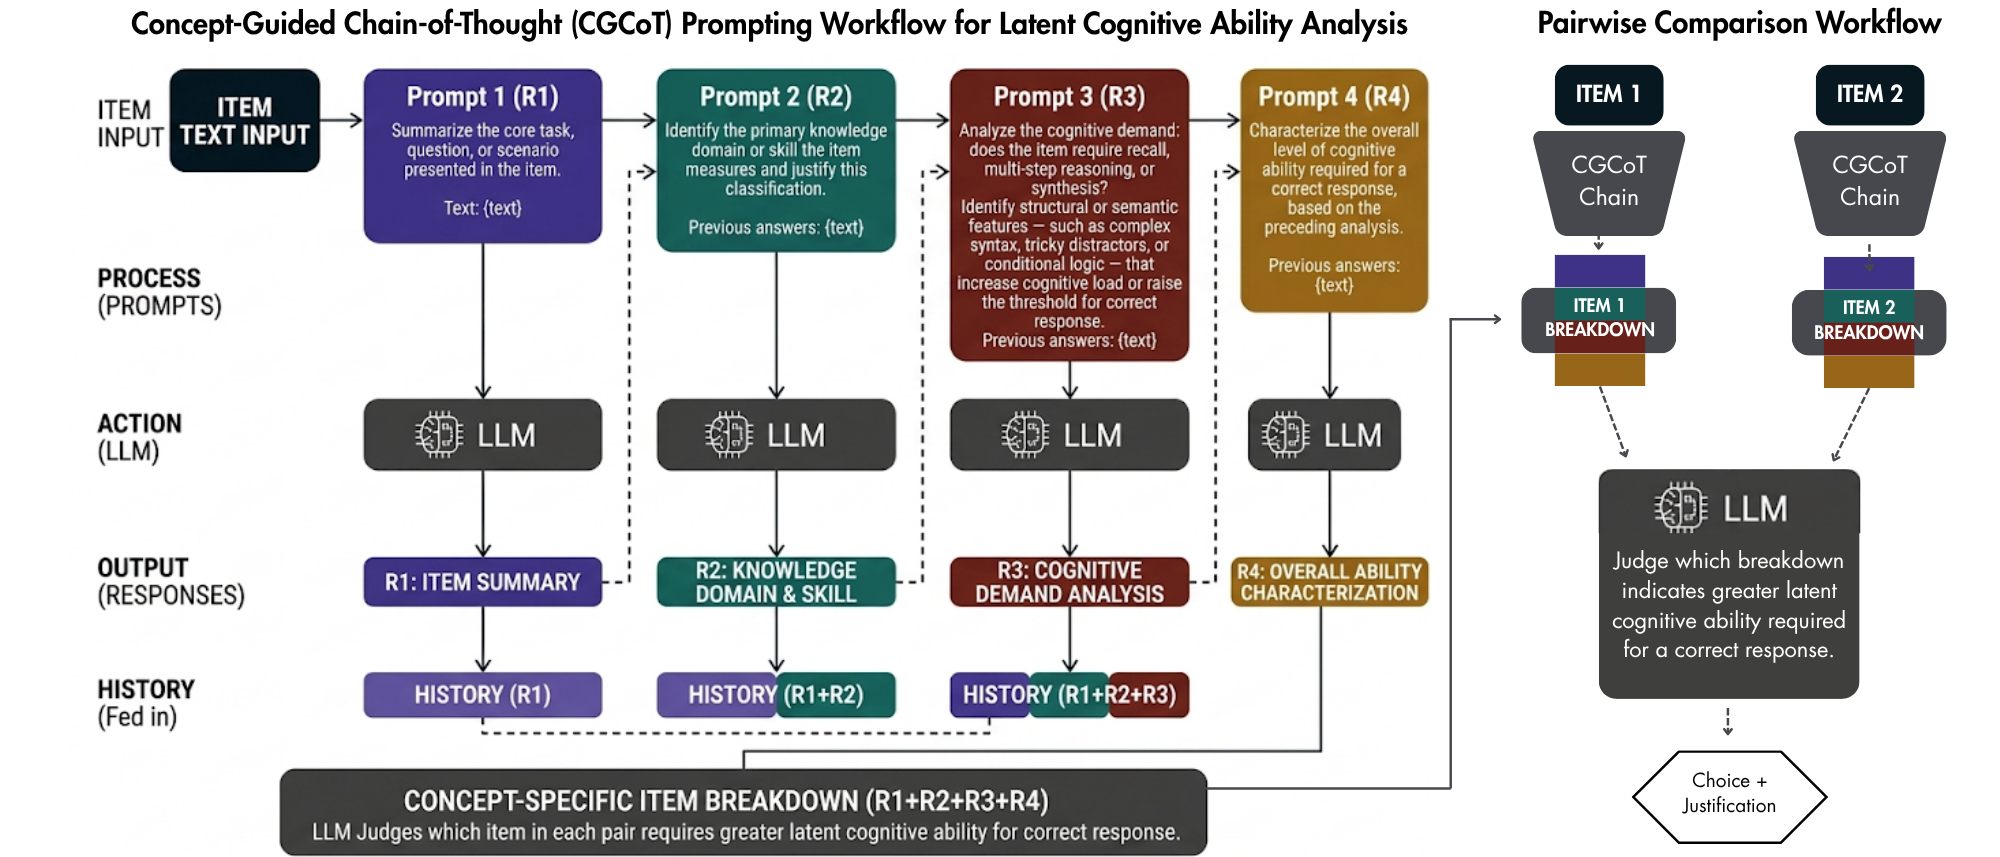
\includegraphics[width=\textwidth]{tables_and_figures/CGCoT_method_figure.png}
  \caption{Concept-Guided Chain-of-Thought (CGCoT) Prompting for Item Difficulty Assessment. Each item is processed through a sequence of four prompts, each targeting a different facet of the latent construct of interest, here item difficulty. The LLM's responses are concatenated and fed into the next prompt, culminating in a comprehensive analysis of the item's difficulty before pairwise comparisons are made.}
  \label{fig:cgcot_method}
\end{figure*}

Seven proprietary LLM configurations served as raters: (\textbf{1}) GPT-5.4 Mini, (\textbf{2}) GPT-5.4, (\textbf{3}) GPT-5.6-Luna, (\textbf{4}) GPT-5.6-Sol, (\textbf{5}) Gemini 3 Flash Preview, (\textbf{6}) Gemini 3.7 Flash, and (\textbf{7})Gemini 3.1 Pro Preview. The panel was selected to vary along three dimensions relevant to the robustness of LLM-based measurement. First, it includes two independently developed model families, OpenAI's GPT and Google's Gemini, reducing the extent to which the findings depend on the idiosyncrasies of a single provider. Second, it includes differently positioned product tiers and variants within each family---Mini and standard GPT-5.4, Luna and Sol variants of GPT-5.6, and Flash and Pro Gemini models---allowing us to examine whether pairwise judgments remain consistent across models marketed for different capability, latency, and cost tradeoffs. Third, the numbered releases within both families broaden the evaluation beyond a single model generation or temporal snapshot. Because the providers do not disclose directly comparable parameter counts, training corpora, or complete architectural details for these proprietary systems, we treat each configuration as a distinct rater rather than interpreting nominal tier or version differences as quantitative measures of model size or capability.

\section{Methods}
\label{sec:methods}

\subsection{\texttt{pairadigm} and Paired Comparisons}
\label{subsec:pairadigm}

All pairwise comparison workflows---CGCoT prompt chaining, comparison management, and BT model estimation---were implemented using \texttt{pairadigm} \citep{chrzanPairadigm}, an open-source Python package for using LLMs to measure scalar constructs. The package includes code for generating pairs from the set of items and applying CGCoT prompts to construct item breakdowns. Using evidence from \citet{wuConceptGuidedChainofThoughtPrompting2024} that beyond 10 pairs per item yielded minimal improvement, where possible we limit the number of possible pairs to 10 per item for compute and cost considerations. The seven configurations listed previously were evaluated as separate comparison judges, enabling rater-specific estimates of consistency, discrimination, and position bias.

For each item, a four-prompt CGCoT chain was administered sequentially to the LLM to target cognitive item difficulty. After the LLM answers each prompt, its response is concatenated to all its previous responses and fed into the next prompt until at the end an entire breakdown of the item is created, as displayed in Figure \ref{fig:cgcot_method}. Prompts are also listed out in Appendix \ref{app:prompts}. 

The resulting concept-specific breakdown for each item was used to generate pairwise comparisons across all item pairs within each dataset. Based on the cumulative output from these four steps applied to an item, the LLM judged which item in a pair required greater latent cognitive ability for correct response. 

\subsection{(Hierarchical) Bradley-Terry Models}
\label{subsec:bradley-terry}

Individual BT models were fit to each LLM`s pairwise preference data for each dataset to produce a continuous BT difficulty score for each item. Triplet transitivity, or the proportion of triplets (A, B, C) in which the model's pairwise judgments were logically consistent, was computed as an additional consistency check. Inter-rater agreement across LLMs was estimated using Krippendorff's Alpha \citep{hayesAnsweringCallStandard2007} to assess the consistency across models for a given IRW dataset. Finally, convergent validity was assessed via Spearman rank correlations computed between each model's BT scores and the corresponding 1PL difficulty parameters, stratified by model and dataset \citep{spearmanProofMeasurementAssociation1904}. Relationships among reliability, inter-rater agreement, and Spearman correlations were examined to assess the relationships between internal consistency and external validity.

A Hierarchical Bradley-Terry model was also fit to assess each LLM`s discrimination and position bias. We formulate the model as follows:

\[
\text{logit}P(y_{ijk} = 1) = \alpha_k(\lambda_i - \lambda_j) + \gamma_k
\]

where 
\begin{itemize}
  \item $y_{ijk} = 1$ indicates that model $k$ selects the first presented item, $i$, over the second-presented item, $j$,
  \item $\lambda_i$ and $\lambda_j$ are the difficulty parameters for items $i$ and $j$,
  \item $\alpha_k$ is the discrimination parameter for participant $k$,
  \item $\gamma_k$ is the position bias for participant $k$.
\end{itemize}

We enforce that (1) the sum of $\lambda_i$ across all items is zero, and (2) the geometric mean of $\alpha_k$ across all models is one, which identifies the global $\alpha-\lambda$ scale without choosing an arbitrary reference model. We discuss the full model details in Appendix \ref{app:bradley_terry}, including the hierarchical priors for $\lambda_i$, $\alpha_k$, and $\gamma_k$. We also structure the data such that every unordered pair is evaluated in both orientations, which balances item identity across first and second positions and makes $\gamma_k$ estimable from direct orientation reversals. 

\subsubsection{Sensitivity Check}
\label{subsubsec:sensitivity_check}

The primary model gives every model judgment equal weight. A provider-balanced sensitivity model weights observations so Google and OpenAI contribute equal total likelihood mass. Additional leave-one-model-out fits test whether item rankings depend strongly on any single model. These are discussed in Appendix \ref{app:sensitivity}.

\section{Results}
\label{sec:results}

\begin{figure*}[t]
  \centering
  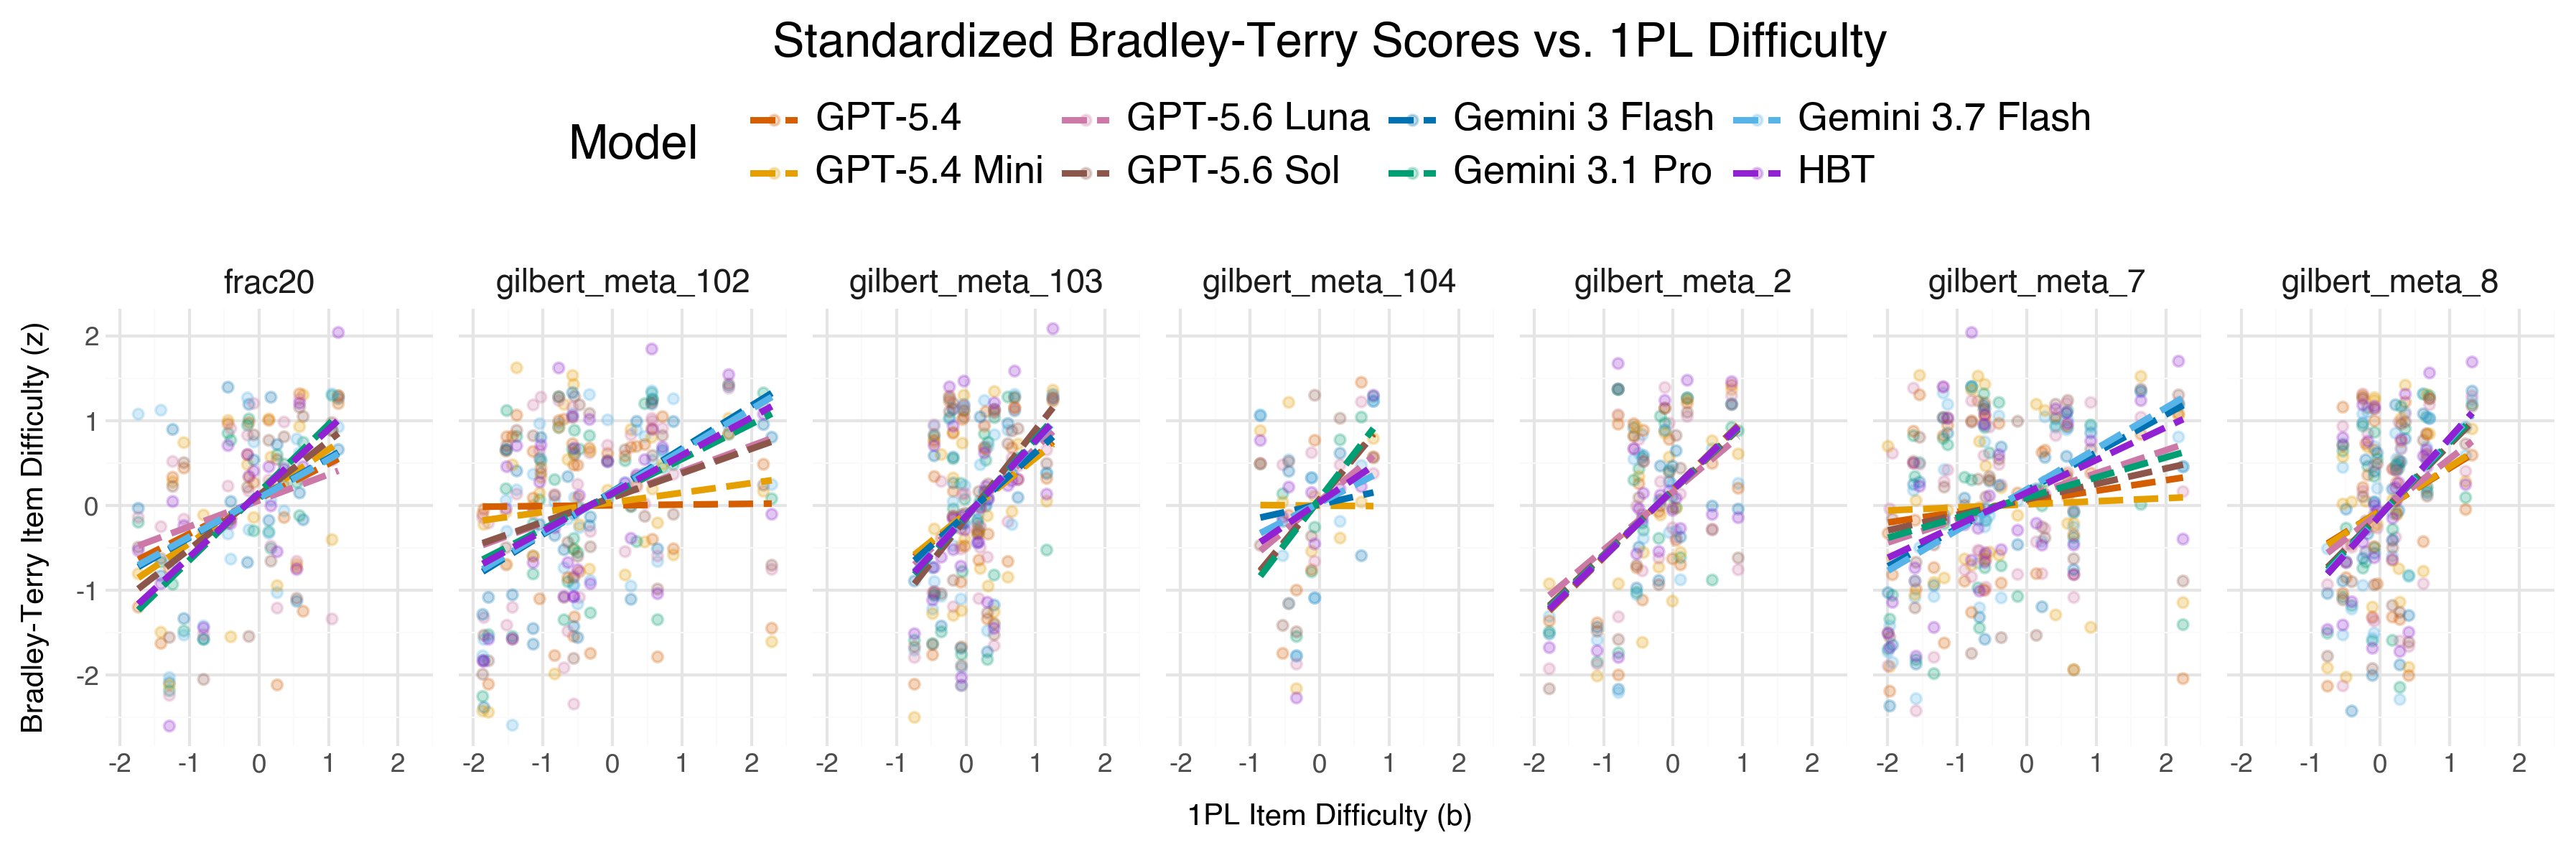
\includegraphics[width=\textwidth]{tables_and_figures/standardized_bt_vs_1pl_by_table.png}
  \caption{Standardized Hierarchical Bradley-Terry Strengths vs. 1PL IRT Difficulty Parameters. Each point represents an item, with the y-axis showing the standardized BT strength estimated from LLM pairwise comparisons and the x-axis showing the corresponding 1PL IRT difficulty parameter. The dashed lines indicates the correlational relationship between the two measures for a given model, illustrating varying degrees of alignment between LLM-derived BT scores and psychometrically validated IRT difficulties.}
  \label{fig:bt_v_1pl}
\end{figure*}


\begin{figure*}[t]
  \centering
  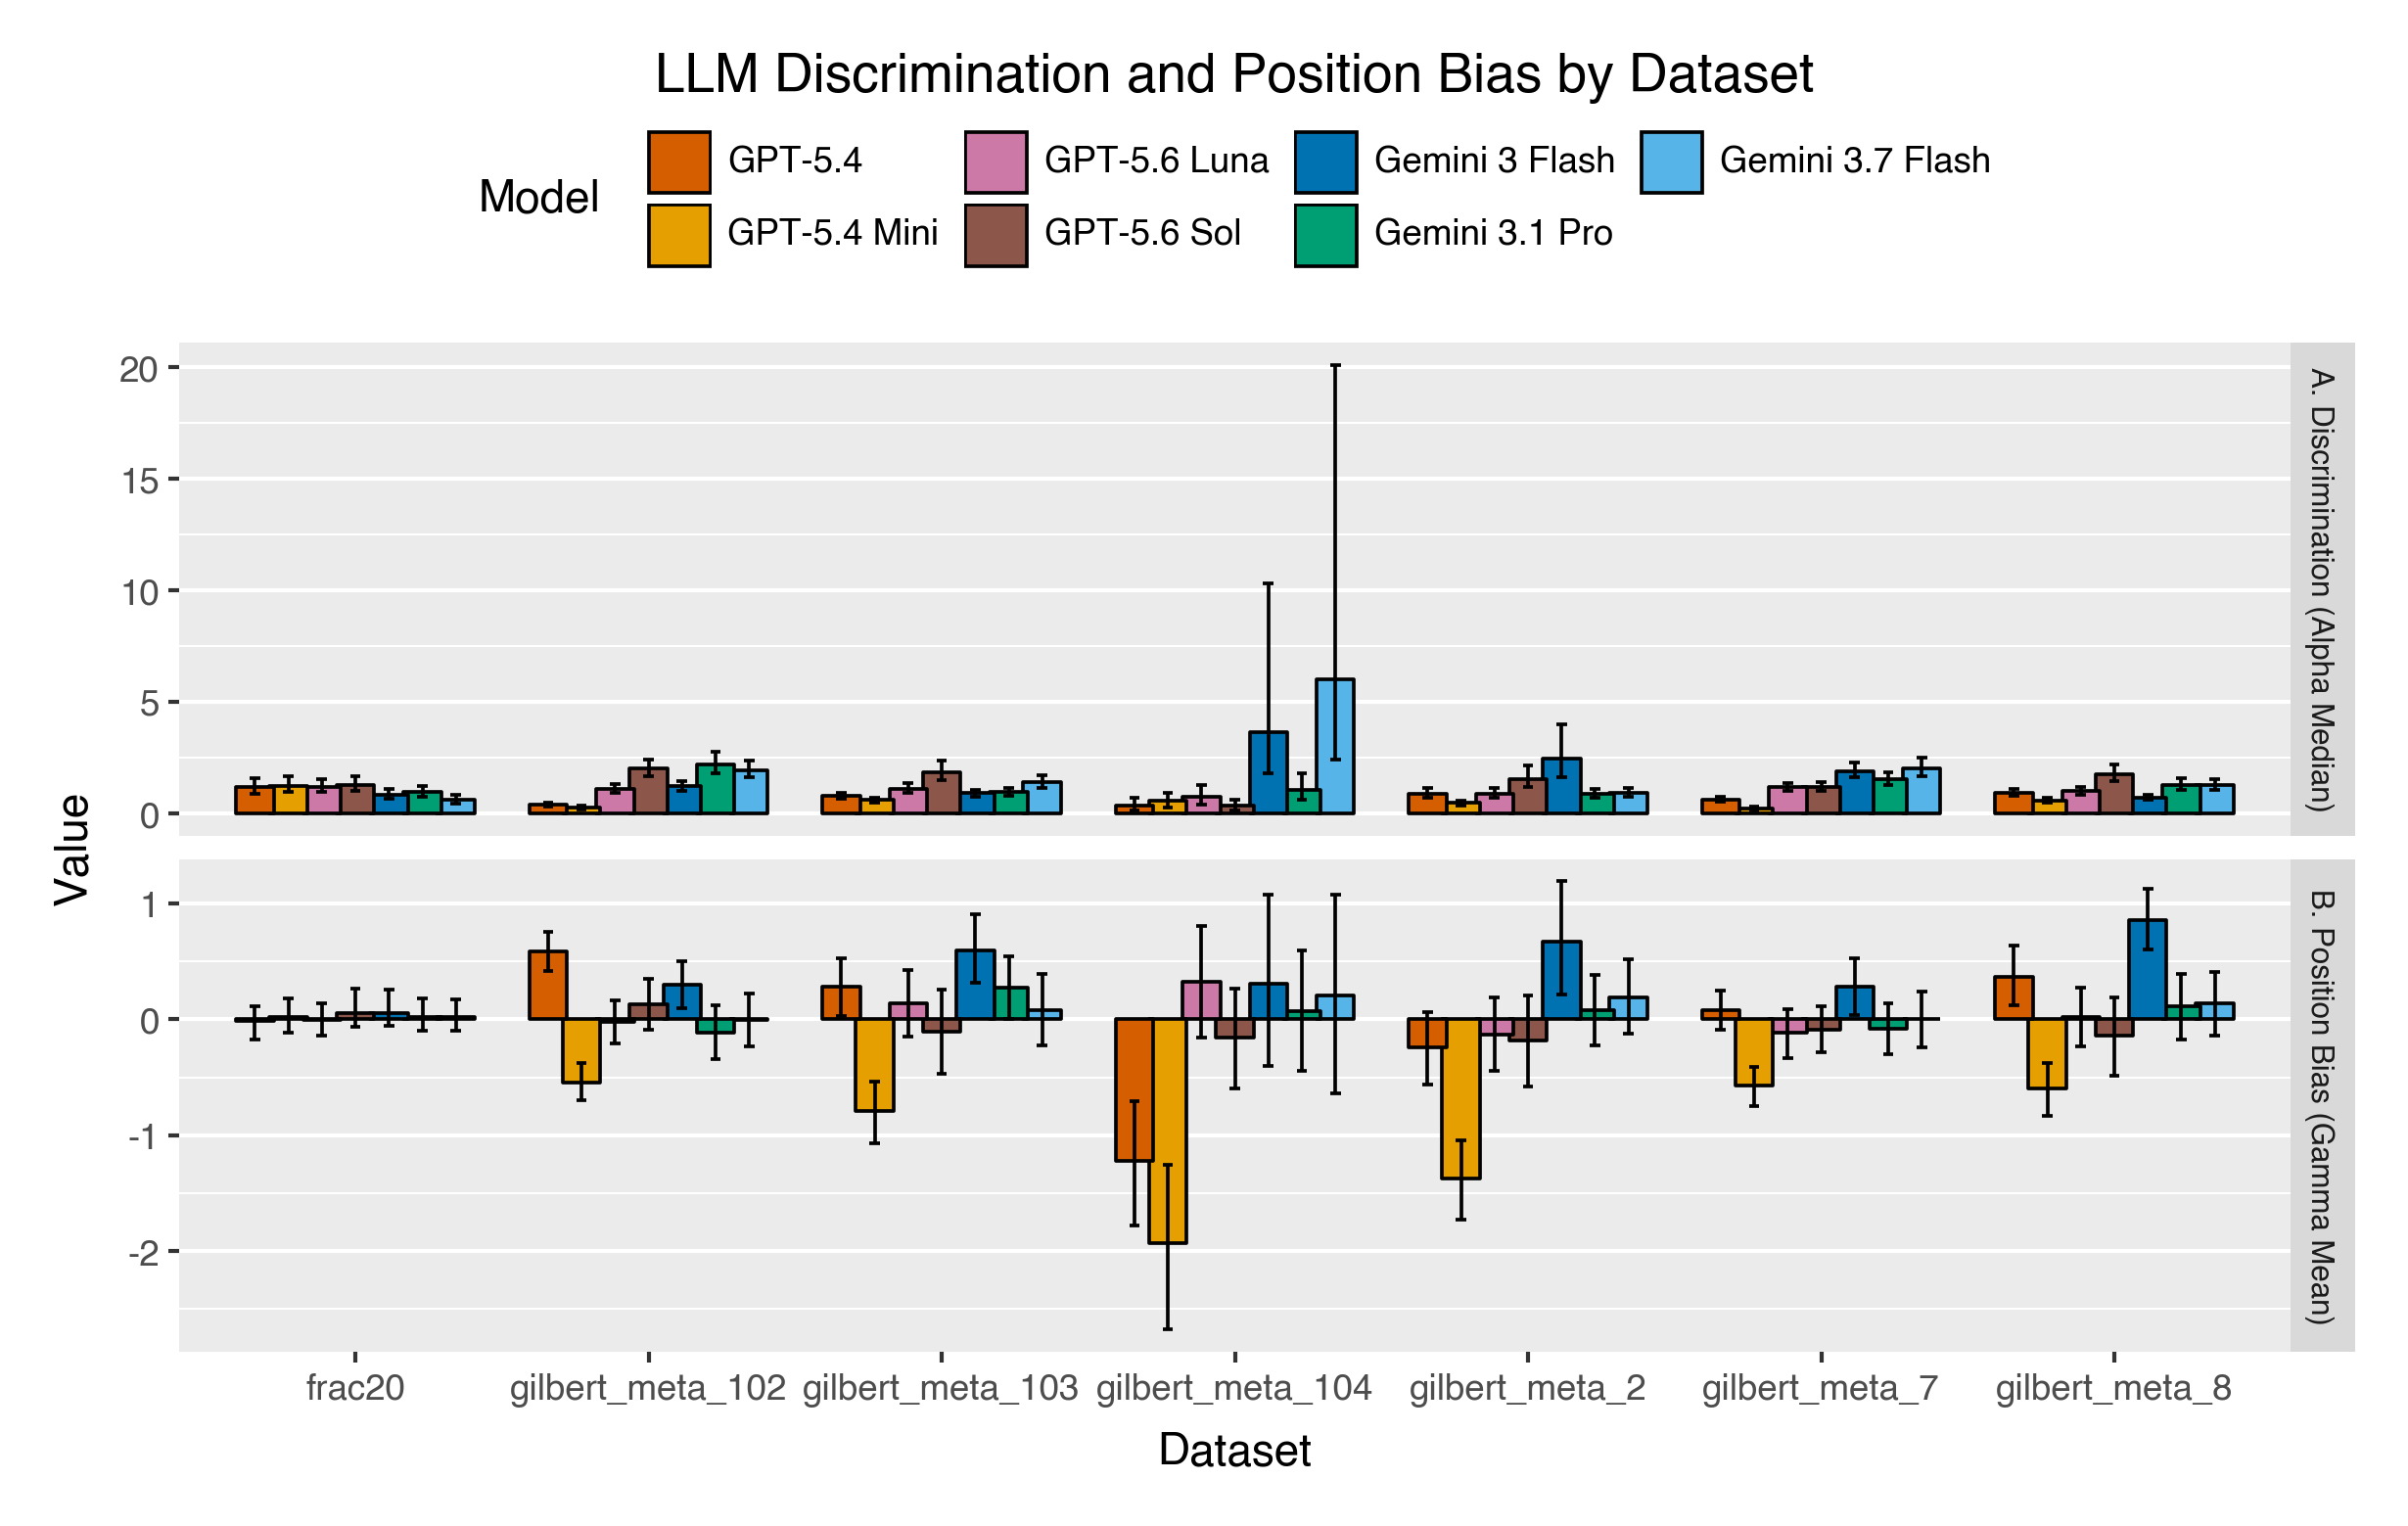
\includegraphics[width=\textwidth]{tables_and_figures/discrim_and_position.png}
  \caption{Discrimination and Position Bias of LLMs. The figure shows the discrimination (Alpha) and position bias (Gamma) of different LLM raters across various datasets. Higher alpha values indicate stronger rater ability to distinguish strength between items, while positive gamma values suggest a bias toward the first item shown. Error bars represent 94\% highest density intervals (HDI) for each estimate. The results highlight the variability in LLM performance across datasets, with some models exhibiting higher discrimination and lower position bias, suggesting better reliability and less susceptibility to order effects in pairwise comparisons.}
  \label{fig:discrim_and_position}
\end{figure*}

\section{Discussion}
\label{sec:discussion}

\section{Conclusion}
\label{sec:Conclusion}

encoders are better, The performance notably fell short of simpler, encoder-only models like ConvBERT utilized with a linear scheduler, which achieved a superior QWK of 0.62510 \citep{wangCanLLMsReally2026}.

\section*{Limitations}
\label{sec:limits}

\begin{itemize}
  \item datasets were restricted to those with available item text in the IRW, which is growing but still limited. Future work should expand to additional datasets and domains to assess generalizability.
  \item The LLMs evaluated are proprietary and subject to change, which may limit reproducibility. Future work should include open-source models and document model versions and configurations. As the number of both models and datasets grows, future work could also explore relationships between model characteristics and performance.
  \item The hierarchical Bradley-Terry model assumes a specific parametric form for discrimination and position bias. Alternative modeling approaches could be explored to assess robustness of the findings.
  \item The study does not examine the impact of prompt design on LLM judgments. Future work could systematically vary prompts to assess sensitivity to prompt wording and structure.
\end{itemize}

\section*{Acknowledgments}
\label{sec:acknowledgments}

\textbf{ASK BEN!}

%Please see Section~\ref{sec:bibtex} for information on preparing Bib\TeX{} files.
%
%\section{Bib\TeX{} Files}
%\label{sec:bibtex}
%
%Unicode cannot be used in Bib\TeX{} entries, and some ways of typing special characters can disrupt Bib\TeX's alphabetization. The recommended way of typing special characters is shown in Table~\ref{tab:accents}.
%
%Please ensure that Bib\TeX{} records contain DOIs or URLs when possible, and for all the ACL materials that you reference.
%Use the \verb|doi| field for DOIs and the \verb|url| field for URLs.
%If a Bib\TeX{} entry has a URL or DOI field, the paper title in the references section will appear as a hyperlink to the paper, using the hyperref \LaTeX{} package.
%
% ---------------------------------------------

% Custom bibliography entries only
\bibliography{custom}

\appendix

\section{CGCoT Prompts}
\label{app:prompts}
The prompts used were:  

\begin{itemize}
  \item "Summarize the core task, question, behavioral statement, or scenario presented in this item. Item text: \{text\}".
  \item "Identify the primary knowledge domain, skill, clinical symptom, attitudinal belief, or psychological construct this item is attempting to measure and give a concise justification. Text: \{text\}"
  \item "Analyze the demand or severity of this item. For cognitive/ability items, does it require recall, multi-step reasoning, or synthesis? For psychological/attitudinal items, does endorsing it require a severe level of a symptom, a strongly held belief, or deep introspection? CONCISELY identify any structural or semantic elements—such as complex phrasing, tricky distractors, conditional logic, or strong emotional wording—that increase the cognitive load or the threshold for endorsement. Text: \{text\}"
  \item "Based on your analysis, describe the overall level of the underlying latent trait (e.g., high cognitive ability, severe psychological symptomology, strong attitude) required for a respondent to successfully answer or strongly endorse this item. Previous analysis: \{text\}"
\end{itemize}

\section{Hierarchical Bradley-Terry Model Details}
\label{app:bradley_terry}

\subsection{Item Difficulty}
\label{appsubsec:item_parameters}
The model estimates a single $\lambda_i$ for each item across all LLMs, allowing us to pool information across models while accounting for model-specific discrimination and position bias. These item strengths are centered to remove translation invariance: 

\[
\begin{aligned}
\lambda_i &= \sigma_{\lambda}(z_i - \bar{z}) \\
u_k &\sim \text{N}(0, 1) \\
\sigma_{\lambda} &\sim \text{HalfNormal}(1)
\end{aligned}
\]

Thus $\sum_i{\lambda_i} = 0$. $\sigma_{\lambda}$ is the standard deviation of the item strengths, $z_i$ is a latent standard-normal random effect, and $\bar{z}$ is the mean of the $z_i$ across all items,

\subsection{Rater Position Bias}
\label{appsubsec:rater_position_bias}

Another way to conceptualize $\gamma_k$ is a measure of model $k$'s tendency to prefer the first item \textit{regardless} of item strength. We model $\gamma_k$ hierarchically, allowing for partial pooling across models and estimating the overall distribution of position bias:

\[
\begin{aligned}
\gamma_k &= \sigma_{\gamma}v_k \\
v_k &\sim \text{N}(0, 1) \\
\sigma_{\gamma} &\sim \text{HalfNormal}(0.5)
\end{aligned}
\]

where $\sigma_{\gamma}$ is the standard deviation of the position bias across models and $v_k$ is a latent standard-normal random effect.

\subsection{Rater Discrimination}
\label{appsubsec:rater_discrimination}

The discrimination parameter $\alpha_k$ captures the ability of model $k$ to distinguish between items of different strengths. We model $\alpha_k$ hierarchically, allowing for partial pooling across models and estimating the overall distribution of discrimination:

\[
\begin{aligned}
\text{log}(\alpha_k) &= \sigma_{\text{log}{\alpha}}(u_k - \bar{u}) \\
u_k &\sim \text{N}(0, 1) \\
\sigma_{\text{log}(\alpha)} &\sim \text{HalfNormal}(0.5)
\end{aligned}
\]

where $\sigma_{\text{log}(\alpha)}$ is the standard deviation of the discrimination across models and $u_k$ is a latent standard-normal random effect.

Centering log discrimination enforces

\[
\text{exp}(\frac{1}{K} \sum_{k} \text{log}(\alpha_k)) = 1
\]

so the geometric mean rater discrimination is one. This identifies the global $\alpha-\lambda$ scale without choosing an arbitrary reference model.

\section{Sensitivity Analyses}
\label{app:sensitivity}

put description of sensitivity analyses here

\end{document}
